% ==================
% Standalone support
% ==================


\makeatletter
\ifdefined\preloaded
\else
	\newcommand{\preloaded}{not set!}
	\ifx\documentclass\@twoclasseserror % after \documentclass
		\renewcommand{\preloaded}{true}
	\else
		\documentclass[12pt]{report}

% Packages
% ========
\usepackage[letterpaper, portrait, margin=1in]{geometry}
\usepackage{graphicx}			% So we can load figures with "." in their filename
\usepackage{float}				% So we can use "[H]"
\usepackage[dvipsnames]{xcolor}	% For custom colors
\usepackage{xparse}				% For \DeclareDocumentCommand
\usepackage{caption}			% For \captionof command
\usepackage{mathtools}			% For \DeclarePairedDelimeter
\usepackage{ifthen}				% For \ifthenelse{}{}{}
\usepackage{soul}				% For underlining with \ul
\setuldepth{x}					%	""
\usepackage{multicol}			% For multiple columns via \begin{multicols}{2}
\usepackage[most]{tcolorbox}	% For the tl; dr environment
\usepackage{array}				% For extended column definitions
\usepackage{tabularray}			% For \begin{longtblr} tables that span multiple columns and pages
\usepackage{amssymb}			% For $\checkmark$
\usepackage{etoc}				% For \localtableofcontents


% Inserting code into LaTeX: \begin{lstlisting} ...
\usepackage{listings}
\definecolor{dkgreen}{rgb}{0,0.6,0}
\definecolor{gray}{rgb}{0.5,0.5,0.5}
\definecolor{mauve}{rgb}{0.58,0,0.82}

\lstset{frame=tb,
  language=C++,
  aboveskip=3mm,
  belowskip=3mm,
  showstringspaces=false,
  columns=flexible,
  basicstyle={\small\ttfamily},
  numbers=none,
  numberstyle=\tiny\color{gray},
  keywordstyle=\color{blue},
  commentstyle=\color{dkgreen},
  stringstyle=\color{mauve},
  breaklines=true,
  breakatwhitespace=true,
  tabsize=3
}

% Inline code
\definecolor{darkpink}{rgb}{0.5, 0.0, 0.5}
\newcommand{\code}[1]{\texttt{\color{darkpink}#1}}

% Bibliography
% ============
\usepackage[american]{babel}
\usepackage{csquotes}
\usepackage[style=ieee, backend=biber]{biblatex}
\usepackage{hyperref}
\hypersetup{colorlinks=true, allcolors=black, urlcolor=blue}
\addbibresource{../sources.bib}

% etoc setup
% ==========

\etocsetstyle{section}{}{}{\etocsavedchaptertocline{\numberline{}\etocname}{\etocpage}}{}
\etocsetstyle{subsection}{}{}{\etocsavedsectiontocline{\numberline{}\etocname}{\etocpage}}{}
\etocsetstyle{subsubsection}{}{}{\etocsavedsubsectiontocline{\numberline{}\etocname}{\etocpage}}{}
\etocsetstyle{paragraph}{}{}{\etocsavedsubsubsectiontocline{\numberline{}\etocname}{\etocpage}}{}
\etocsetstyle{subparagraph}{}{}{\etocsavedparagraphtocline{\numberline{}\etocname}{\etocpage}}{}


% Simple custom commands
% ======================
\makeatletter
\def\maxwidth#1{\ifdim\Gin@nat@width>#1 #1\else\Gin@nat@width\fi} 
\makeatother

\def\todo#1{\selectfont{\color{red}\texttt{\textbf{TODO:} #1}}}

% Sections 'n' such
% =================

\definecolor{chaptColor}{RGB}{0, 83, 161}

\def\chapt#1{
%
	% Default chapter behavior
	\begingroup\color{chaptColor}
	\chapter{#1}
	\endgroup
	
	% Label
	\label{chp:#1}
}

\definecolor{sectColor}{rgb}{0, 0.5, 0.0}
\def\sect#1{\textcolor{sectColor}{\section{#1}}}

\definecolor{subsectColor}{rgb}{0, 0.5, 0.5}
\def\subsect#1{\textcolor{subsectColor}{\subsection{#1}}\noindent}

\definecolor{subsubsectColor}{rgb}{0.747, 0.458, 0}
\def\subsubsect#1{\textcolor{subsubsectColor}{\subsubsection{#1}}}

% TL; DR section
% ==============
\newenvironment{tldr}{\begin{tcolorbox}[colback=gray!20!white,colframe=blue!75!black,title=TL; DR]}{\end{tcolorbox}\vspace*{12pt}}

% Custom math commands
% ====================
\DeclarePairedDelimiter\ceil{\lceil}{\rceil}
\DeclarePairedDelimiter\floor{\lfloor}{\rfloor}

% ======================
% \graphic{filename=...}
% ======================
% Keyword arguments
\makeatletter
\define@key{graphicKeys}{filename}{\def\graphic@filename{#1}}
\define@key{graphicKeys}{scale}{\def\graphic@scale{#1}}
\define@key{graphicKeys}{width}{\def\graphic@width{#1}}
\define@key{graphicKeys}{caption}{\def\graphic@caption{#1}}
\define@key{graphicKeys}{captionType}{\def\graphic@captionType{#1}}
\define@key{graphicKeys}{label}{\def\graphic@label{#1}}

% Kwargs
\DeclareDocumentCommand{\graphic}{m}{

	\begingroup
	
	% Set default kwargs
	\setkeys{graphicKeys}{filename={0}, #1}
	\setkeys{graphicKeys}{scale={0}, #1}
	\setkeys{graphicKeys}{width={0}, #1}
	\setkeys{graphicKeys}{caption={}, #1}
	\setkeys{graphicKeys}{captionType={figure}, #1}
	\setkeys{graphicKeys}{label={}, #1}
	
	% Assign width
	\let\graphicWidth\relax % let \mytmplen to \relax
	\newlength{\graphicWidth}
	\setlength{\graphicWidth}{\columnwidth}
	
	\if \graphic@scale 0
		
		\if \graphic@width 0
			
			\setlength{\graphicWidth}{0.5\columnwidth}
		
		\else
	
			\setlength{\graphicWidth}{\graphic@width}
			
		\fi

	\else
		
		\setlength{\graphicWidth}{\columnwidth * \graphic@scale}

	\fi	
	
	% Do figure
	\begin{minipage}{\columnwidth}
		\vspace*{12pt}
		\begin{center}
		
			\includegraphics[width = \graphicWidth]{\graphic@filename}
			
			\ifthenelse{\equal{\graphic@caption}{}}{}{
				\captionof{\graphic@captionType}{\graphic@caption}
			}
			
			\ifthenelse{\equal{\graphic@label}{}}{
				\label{fig: \graphic@filename}
			}{
				\label{\graphic@label}
			}
		\end{center}
		\vspace*{12pt}
	\end{minipage}
	
	\endgroup
}
\makeatother

% ==============
% Base Pair Page
% ==============
% Keyword arguments
\makeatletter
\define@key{bpPageKeys}{baseFilename}{\def\bpPage@baseFilename{#1}}
\define@key{bpPageKeys}{scale}{\def\bpPage@scale{#1}}
\define@key{bpPageKeys}{width}{\def\bpPage@width{#1}}
\define@key{bpPageKeys}{caption}{\def\bpPage@caption{#1}}
\define@key{bpPageKeys}{captionType}{\def\bpPage@captionType{#1}}
\define@key{bpPageKeys}{label}{\def\bpPage@label{#1}}

% Kwargs
\DeclareDocumentCommand{\BPPage}{m}{

	\begingroup
	
	% Set default kwargs
	\setkeys{bpPageKeys}{baseFilename={0}, #1}
	\setkeys{bpPageKeys}{caption={}, #1}
	\setkeys{bpPageKeys}{label={}, #1}
	
	\newpage

	\begin{center}
		\ul{\mbox{\bpPage@baseFilename{}: 1 Base Pair [min]}}
	\end{center}
	\vspace*{-36pt}
	\begin{minipage}[b]{0.5\textwidth}
		\graphic{filename=\bpPage@baseFilename-overview-1-table, width=\textwidth}
	\end{minipage}
	\begin{minipage}[b]{0.5\textwidth}
		\graphic{filename=\bpPage@baseFilename-overview-1-plot, width=\textwidth}
	\end{minipage}

	\begin{center}
		\ul{\mbox{\bpPage@baseFilename{}: 50 Base Pairs [average]}}
	\end{center}
	\vspace*{-36pt}
	\begin{minipage}[b]{0.5\textwidth}
		\graphic{filename=\bpPage@baseFilename-overview-50-table, width=\textwidth}
	\end{minipage}
	\begin{minipage}[b]{0.5\textwidth}
		\graphic{filename=\bpPage@baseFilename-overview-50-plot, width=\textwidth}
	\end{minipage}
	
	\begin{center}
		\ul{\mbox{\bpPage@baseFilename{}: 100 Base Pairs [max]}}
	\end{center}
	\vspace*{-36pt}
	\begin{minipage}[b]{0.5\textwidth}
		\graphic{filename=\bpPage@baseFilename-overview-100-table, width=\textwidth}
	\end{minipage}
	\begin{minipage}[b]{0.5\textwidth}
		\graphic{filename=\bpPage@baseFilename-overview-100-plot, width=\textwidth}
	\end{minipage}

	\vspace*{-24pt}
	\captionof{figure}{\bpPage@caption}\label{\bpPage@label}	
	
	\endgroup
}
\makeatother



\begin{document}
  		\begin{document}
		\renewcommand{\preloaded}{false}
	\fi
\fi
\makeatother
\trysetmain{}

% Additional usage: \ifthenelse{\equal{\preloaded}{true}}{ ... }{ ... }
% Note: Cannot do \trysetmain{} here because the \currfilename will always be "standalone.tex"
% ================================
% Effect table environment. Usage:
%	\begin{OutletTable}{Base Effect Class}
%		...
%	\end{OutletTable}
%
%	- Effect -> UEffectComponent automatically
% ================================
\newenvironment{EffectTable}[1]{%
\begin{longtblr}[
	caption = {All \code{U#1Component}s currently implemented and tested.},
	label = {#1-table},
]{
		colspec={Q[l, wd=0.17\textwidth] Q[l, wd=0.22\textwidth] Q[l, wd=0.25\textwidth] Q[l, wd=0.11\textwidth] Q[l, wd=0.19\textwidth]},
		hlines,
		row{1} = {font=\bfseries, fg=ICBlue},
		colsep = 0.005\textwidth,
}
	#1  		& Short Description	& Implemented via & Priority	& Note\\
}{%
\end{longtblr}
}



%--------------------------

\code{DependentEffectComponent}s add common, cross-class functionality to other effects. Any \\\code{DependentEffectComponent}:

\begin{itemize}
	\item{has an \code{Owner} that it's dependent upon.}
	\item{is automatically added just after its \code{Owner} is added.}
	\item{is automatically destroyed just before its \code{Owner} is destroyed. This also happens if the dependent is unregistered.}
	\item{follows its \code{Owner}'s \code{Silence} and \code{Unsilence}.}
	\item{returns its \code{Owner}'s \code{Priority}, \code{Stacks}, \code{MaxStats}, \code{Priority}, and \code{ShouldApplyEffect}.}
	\item{is not visible to UI.}
\end{itemize}

\subsection{Concrete Example}

For example, both \code{BerserkerGene} (a \code{Mutation}) and \code{FullBloom} (a \code{PositiveAura}) modify stats. Despite being different inheritance hierarchically, they do pretty similar things. They utilize \code{PermStatMod}. For this example, 
\begin{itemize}
	\item{The \code{EffectComponent} is \code{BerserkerGene}\\
		\hspace*{2em}$\drsh{}$+15\%PhA $|$ -10\% PhD $|$ -10\%SpD}
	\item{The \code{DependentEffectComponent} is \code{PermStatMod}}
\end{itemize}
To attach \code{PermStatMod} to \code{BerserkerGene}, add the following to \code{BerserkerGene::OnComponentCreated}:

\begin{center}
	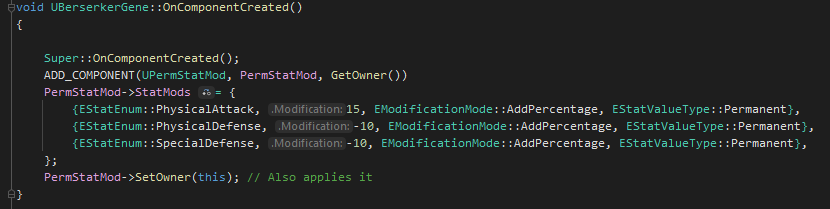
\includegraphics[scale=\ScreenshotScale]{dependent-add}
\end{center}

\newpage

You can also initialize things on the \code{PermStatMod} side of things. For example, if you wanted to make sure there were stats attached to the new owner:

\begin{center}
	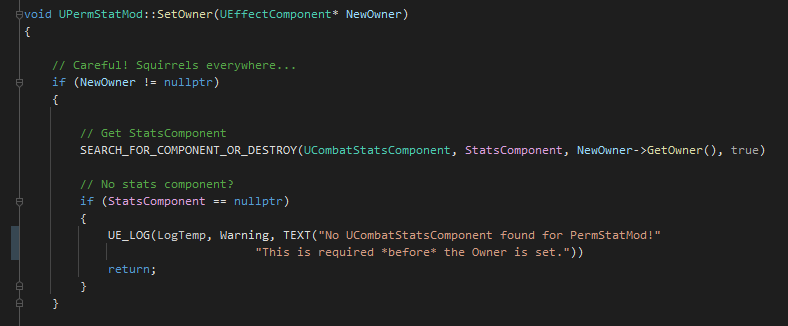
\includegraphics[scale=\ScreenshotScale]{dependent-customization}
\end{center}

\subsection{List of \code{DependentEffectComponent}s}

\begin{EffectTable}{Dependent}
	PermStatMod	& {Modifies \code{EStatEnum}s according to its \code{TArray} of \code{FStatMod}s.}	& \code{AfterRecalculateStats} & \textit{Dependent} & See, e.g., \code{BerserkerGene}.\\
\end{EffectTable}

%--------------------------

\postamble{}